\note{Brief Overview}{
	The first two CLASP Activities in this DLM continue \hyperref[dlm2]{DLM\ref*{dlm2}} with the qualitative study of both the \ThreePhaseModel{} and the \EnergyInteractionModel{}. They extend the work you did on the FNTs assigned at the end of \hyperref[dlm2]{DLM\ref*{dlm2}}.
	
	The last CLASP Activity begins \texttt{Module 1.2}: Getting Quantitative with Models.
	
	\subsubsection*{If you run out of time to complete DL Activities}
	
		In general, for any unfinished DL activities from the previous DL (which should have been assigned as an FNT), give a brief summary (\textless \unit[5]{min}) at the beginning of the current DL and sum up the main points for them. Don't spend time in DL as you normally would having the students discuss and explain.
	
	\subsubsection*{Instructor notes}
	
		Read the instructor notes before the TA meeting!! They contain not only answers (to most of the questions), but also information about what the students should be getting out of the activity, and, at times, instructions on how to run the activity. Be prepared to ask questions in the DL meeting to clarify anything you are not sure of, e.g., ``What is important for the students to get from this?''
		
	\subsubsection*{FNTs}
	
		This is the first time the students will see what they are expected to do with the FNTs. Specifically, they all should have worked hard on them outside of class. Then, in their small groups, they will have the opportunity to clear up their uncertainties about making \EnergyDiagrams{} and using them to make sense of physical phenomena. You should ``check off'' the FNTs or in some way note which of your students have put in an acceptable amount of effort working on them and which have not. Students need to know that you are keeping a record of whether they are doing their homework or not. What's important is that they work on the FNTs, not that they ``get them exactly right'' when they first do them.
		
	\subsubsection*{Explanations on the board}
	
		Students are often asked to write explanations in words on the board. Encourage them to outline, abbreviate, paraphrase, use sentence fragments, etc. in order to reduce the time required to write those explanations. In other words they don't have to be quite as careful in producing explanations for WC consumption as they should on exams, because they can easily clarify in the WC discussion.
	
	\subsubsection*{No equipment needed for DLM03}
}

\note{Reminder}{The goal in this course is ``making sense,'' not getting answers.}

\section{Practicing Our Two Models}
\label{act1.1.4}

\begin{overview}

	\noindent
	{\bfseries Overview:} We continue to practice using the \ThreePhaseModel{}, and we'll start to get more familiar with the \EnergyDiagrams{} of the \EnergyInteractionModel{}.

\end{overview}


\note{Timing: \unit[65]{min}}{

	\subsubsection*{Purpose}
		\begin{itemize}
			\item To become more familiar with the \ThreePhaseModel{} and the \EnergyInteractionModel{}, the meaning of the model constructs and the diagrammatic representations of the models
			\item To become more familiar with applying these two models to particular thermal processes
		\end{itemize}
	
	\subsubsection*{Learning Outcome}
		\begin{itemize}
			\item Be able to quickly and confidently apply both the \ThreePhaseModel{} and the \EnergyInteractionModel{} to the kinds of phenomena treated in this activity. This means being able to confidently use the diagrammatic representations of both models to develop explanations and answer specific questions related to these kinds of thermal phenomena.
		\end{itemize}
}

\subsection{Basics of the \ThreePhaseModel{}}

\begin{fnt}
	\label{fnt1.1.1-1}
\subsubsection*{Scientists don't come up with ``right answers.''}

Usually, when your instructor asks you to ``do problems'' for homework or on a test, they expect you to get a ``right answer,'' right? Well, we don't. As a matter of fact, for many of the problems you will encounter in this course, there won't be one ``right answer.'' Science just doesn't work that way. For every problem, there are a number of ways one can approach the problem, and each different solution path might result in different answers. But, that doesn't mean that one of them is ``right'' and the others are not.

\subsubsection*{Scientists come up with arguments.}

Much more important than an answer to a question or problem in science is usually the method by which one arrived at this answer. So, our emphasis is on the method you use to solve a problem. The pathway to your solution. \textbf{We want to know what assumptions and decisions you're making as you solve a problem, and how you're using these assumptions and decisions to \emph{make an argument} for \emph{your} solution.} That's how science works! There is nobody who knows ``the right answer.'' But there are people who can look at what you've done and who can tell you whether the assumptions you've made are appropriate in a particular situation and the argument you've constructed is valid and convincing. In science, this is called ``peer-review'' because the people who look at your work are other scientists.

\subsubsection*{So, if we don't care so much about you ``getting the right answer,'' how will we evaluate your progress in this course?}

Just like in a scientific publication, \textbf{we ask you to be \emph{very specific} about what you did and did not do, and \emph{how} you arrived at a particular solution to a problem.} We'll practice this a lot, so that you know what we expect from you. This first problem is an extreme example of what problem-solving in this class looks like for you: \emph{We'll actually give you some answers.} A little further down, you'll find a box with some answers that one might reasonably get when solving this problem. Note that we're not saying these are the exact answers you will get or that we expect you to get! But your solutions to this problem might be quite similar to the ones given below.

\subsubsection*{Now, if we give you the answers, what do we want you to do?}

We want you to describe in detail how you are using the diagram below to respond to the prompts in the problem. Write a story about the diagram and about how you are reading the graph to get the values you get. While this is stated a few times below, it's worth repeating: \emph{We don't want you to do any calculations for this problem!} Instead, use the diagram and tell us \emph{how} you're using the diagram and \emph{why} we should believe you that your answer to the problem is a reasonable one.

Yes, this might be a bit more work than what you're used to from other classes. Later in this course, we'll find shorter ways for you to show us your work and argument. But for now, \textbf{\emph{please do write out a detailed story -- including your assumptions, decisions, etc. -- for each part of the problem.}}

\subsubsection*{On to the actual problem:}

Use the particular \TempGraph{} of the \ThreePhaseModel{} shown below to respond to the prompts in this FNT.\\

\noindent
{\centering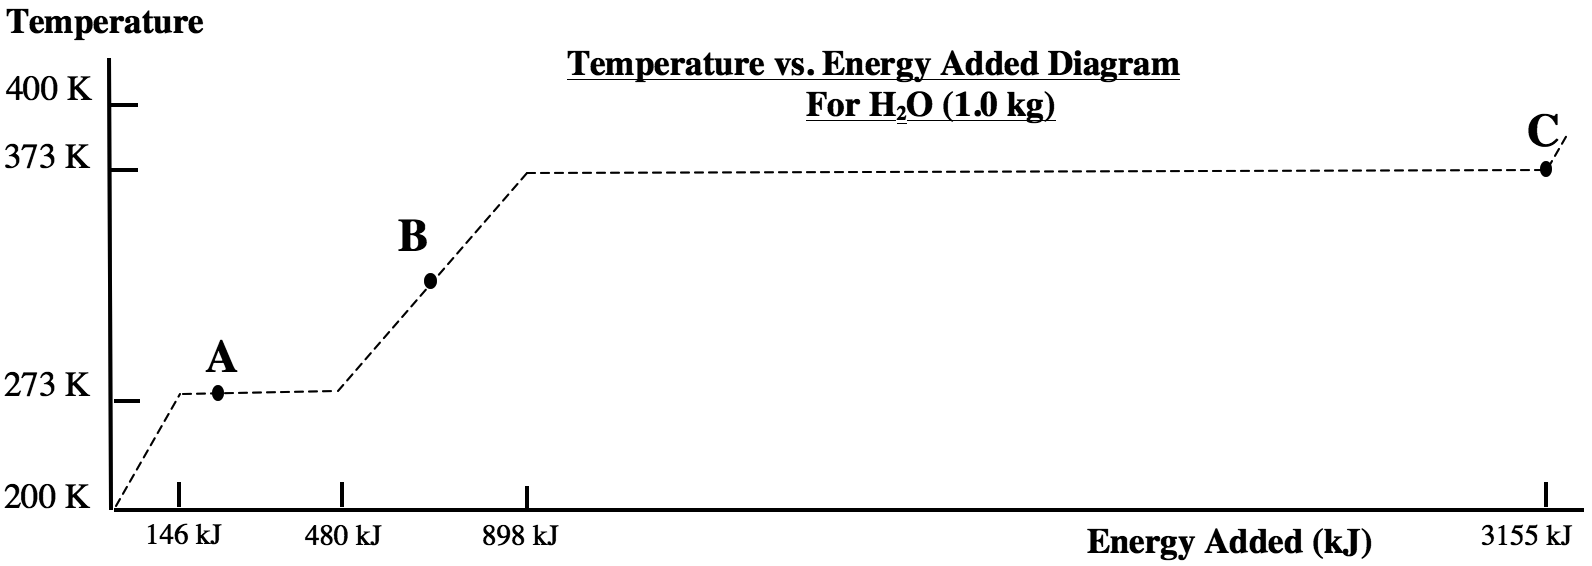
\includegraphics[width=.95\linewidth]{fnt111-1.png}\par}

\noindent The values along the $x$-axis (\unit[146]{kJ}, \unit[480]{kJ}, etc.) are the amounts of energy that must be added to get the \unit[1.0]{kg} of water from an initial temperature of \unit[200]{K} to the next phase change. For example, \unit[480]{kJ} is the total amount of energy that must be added to the water starting at the initial temperature of \unit[200]{K} to completely melt all the ice.

\begin{enumerate}
	\item Describe what is happening at each of the ``corners'' on the graph. What phase is the water in at the letter A, B, C?
	\label{fnt1.1.1-1A}
	
	\item Assume that you have one kilogram of water at an initial temperature of \unit[200]{K}. If \unit[795]{kJ} of energy is added, describe the final state (approximate temperature and phase) of the water. If the water is in a mixed phase, determine very approximately the percent in each phase.
	
		You are not expected to do any calculations at this time. Simply tell us what the diagram tells you (and how you know that it does).
	\label{fnt1.1.1-1B}
	
	\item Repeat \hyperref[fnt1.1.1-1B]{Part~\ref*{fnt1.1.1-1B}} but with \unit[146]{kJ} of energy added to the water initially at \unit[200]{K}.
	
	\item Repeat \hyperref[fnt1.1.1-1B]{Part~\ref*{fnt1.1.1-1B}} but with \unit[1650]{kJ} of energy added to the water initially at \unit[200]{K}.
	
	\item State the initial and final conditions of the process that takes the system from Point C to Point B and determine very approximately how much energy would have to be added or removed.
	\label{fnt1.1.1-1C}
	
	\item Repeat \hyperref[fnt1.1.1-1C]{Part~\ref*{fnt1.1.1-1C}} for water initially in State A and ending in State C.
	\label{fnt1.1.1-1D}
	
\end{enumerate}

\subsubsection*{Again: Do not make any calculations to respond to these prompts!}
\end{fnt}
\note{}{
	Get students started checking their responses to this FNT as they come into the room.
	
	Before the WC discussion, ask each group to put the response to one of the prompts in \#2 of the Activity on the board. Then in the WC discussion, ``randomly'' call on someone from each group to explain how they knew how to respond to that prompt. Emphasize that they really need to know how to use this modeling tool: the \TempGraph{}.
	
	You might also call on someone to explain anything in part \#1 if you feel it is necessary.
}

\noindent
You've all done this FNT individually at home. Now you have an opportunity to practice creating scientific arguments together. Back up your claims with evidence and try to convince each other of \emph{your} solution!

\begin{enumerate}
	\item Discuss with your group and make sure \emph{every} group member is confident that she/he can explain \hyperref[fnt1.1.1-1A]{Question~\ref*{fnt1.1.1-1A}} on the FNT.
	
	\item While there is not one single correct answer for \hyperref[fnt1.1.1-1B]{Parts~\ref*{fnt1.1.1-1B}} -- \hyperref[fnt1.1.1-1D]{\ref*{fnt1.1.1-1D}} of the FNT, you probably estimated the values somewhere in the vicinity of those in the box. Work out in your small groups any significant discrepancies you might have. EVERYONE in your group should be ready to explain how you obtained these results in the whole class discussion. Your instructor will tell your group which prompt you should respond to on the board.
\end{enumerate}

\begin{ans}
	\begin{enumerate}[(a)]
		\item liquid at \unit[$\sim$350]{K}
		\item completely solid at \unit[273]{K}
		\item $\sim$1/3 gas, $\sim$2/3 liquid at \unit[373]{K}
		\item initial conditions: all gas at \unit[373]{K}, final conditions: liquid at \unit[$\sim$50]{\textdegree C}; $\Delta$E~$\approx$~\unit[2470]{kJ}
		\item initial conditions: $\sim$25\% liquid at \unit[0]{\textdegree C}, final conditions: gas at \unit[100]{\textdegree C}; $\Delta$E~$\approx$~\unit[3000]{kJ}
	\end{enumerate}
\end{ans}


\WCD

\subsection{Basics of the \EnergyInteractionModel{}}

%\noindent
%{\bfseries Overview:} Using the \EnergyInteractionModel{} to describe simple processes.

\begin{fnt}
	\label{fnt1.1.3-1}

Neatly write out all of the \EnergyDiagrams{}, with the accompanying \TempGraphs{}, listed below (these are the same scenarios that were requested in \hyperref[act1.1.3]{Activity~\ref*{act1.1.3}}).

Remember that complete \EnergyDiagrams{} always include algebraic expressions of energy conservation. Refer to the \EnergyInteractionModel{} discussion in the online resources.

\begin{enumerate}[(a)]
	\item Cooling a piece of solid copper (Cu) from \unit[500]{\textdegree C} to \unit[350]{\textdegree C}.
	\item Warming a piece of ice from \unit[-20]{\textdegree C} to the melting point.
	\item Condensing steam completely to liquid at \unit[100]{\textdegree C}.
	\item Completely sublimating a chunk of dry ice at \unit[-79]{\textdegree C}.
	\item Partially melting 25\% of ice initially at \unit[0]{\textdegree C}.
	\item Heating a piece of copper initially at \unit[300]{\textdegree C} until it is half melted.
	\item Cooling and completely freezing H$_2$O initially at \unit[80]{\textdegree C}.
\end{enumerate}


\end{fnt}
\note{}{
	{\em Stress} to the WC that they should have little trouble with these. They need to look at ``General Process of Constructing an \EnergyDiagram{}'' and quickly compare with each other. Give no more than \unit[5]{min} to do their comparing.
	
	You can ask if there are any issues the entire SG is unsure of, and then respond to the WC very briefly.
}

\begin{enumerate}
	\item Compare your responses for the processes in \hyperref[act1.1.3]{Activity~\ref*{act1.1.3}}, both the \TempGraphs{} and the \EnergyDiagrams{}.
	
	\item Your instructor will tell you which one of the scenarios (a) through (g) to put on the board.
		
	Put the \TempGraph{} and the \EnergyDiagram{} near each other. Make sure the two diagrams are consistent with each other and make sure everyone in the group can explain precisely why both are drawn the way you have them.

\WCD

\end{enumerate}
